\section{内骨格型グリッパ}
本研究で用いた内骨格型グリッパを\refig{gripper}に示す.内骨格部分が左右に開閉する並行チャック式である.

\begin{figure}[b]
 \begin{center}
  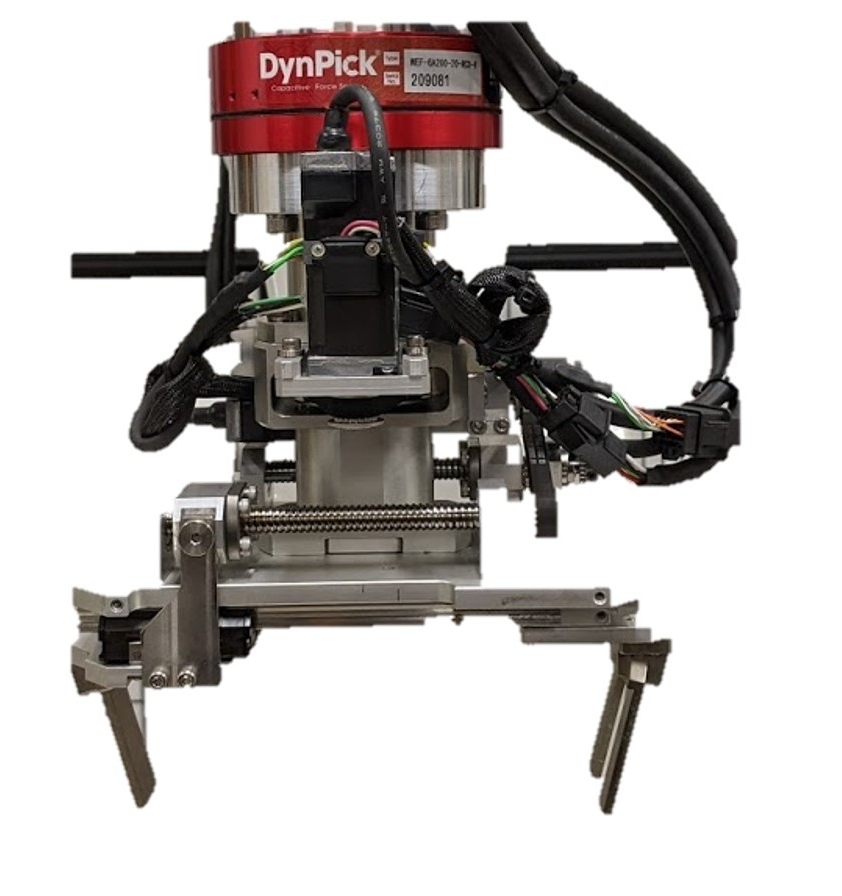
\includegraphics[scale=0.4]{../fig/eps/gripper.eps}
 \caption{内骨格型グリッパ}
  \label{fig::gripper}
 \end{center}
\end{figure}


\subsection{柔軟指}
本研究で提案する柔軟指2種類ある.どちらの指も柔軟な把持部にラティス構造を有している.ラティス構造に関しては次の項目で詳しく述べる.3Dプリンタで作成した.使用した3DプリンタはKEYENCE製AGILISTA-3200(\refig{agilista})を用いた.材質はAR-G1H(高硬度シリコン)とした.

\begin{figure}[b]
 \begin{center}
  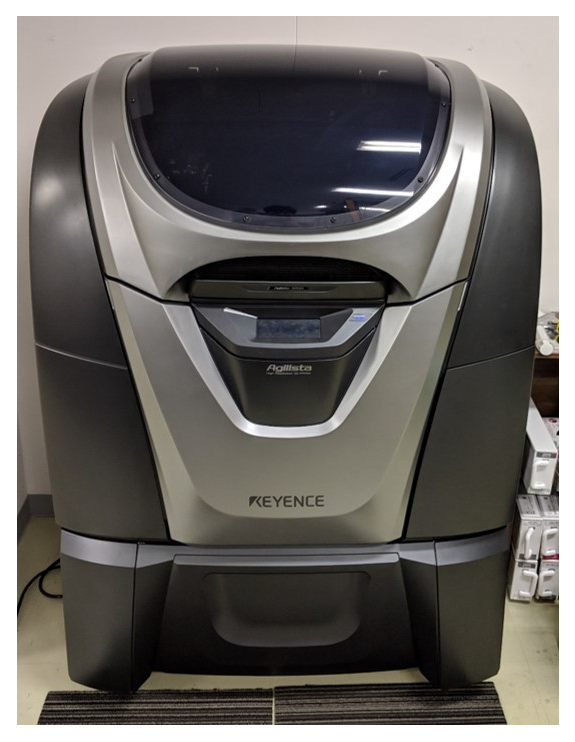
\includegraphics[scale=0.4]{../fig/eps/agilista.eps}
 \caption{KEYENCE製AGILISTA-3200}
  \label{fig::agilista}
 \end{center}
\end{figure}

\subsubsection{通常柔軟指}
通常柔軟指を\refig{soft_finger}に示す.

\begin{figure}[h]
\centering
\subfloat[正面]{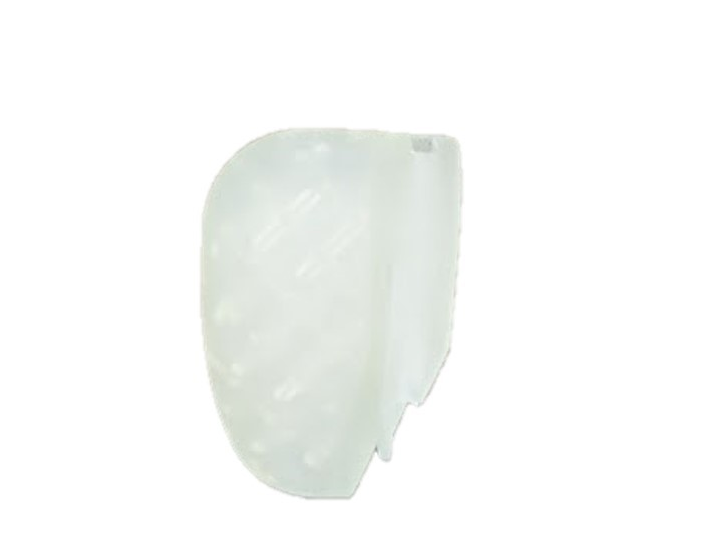
\includegraphics[scale=0.4]{../fig/eps/soft_fingerB.eps}}
\hspace{5mm}
\subfloat[横]{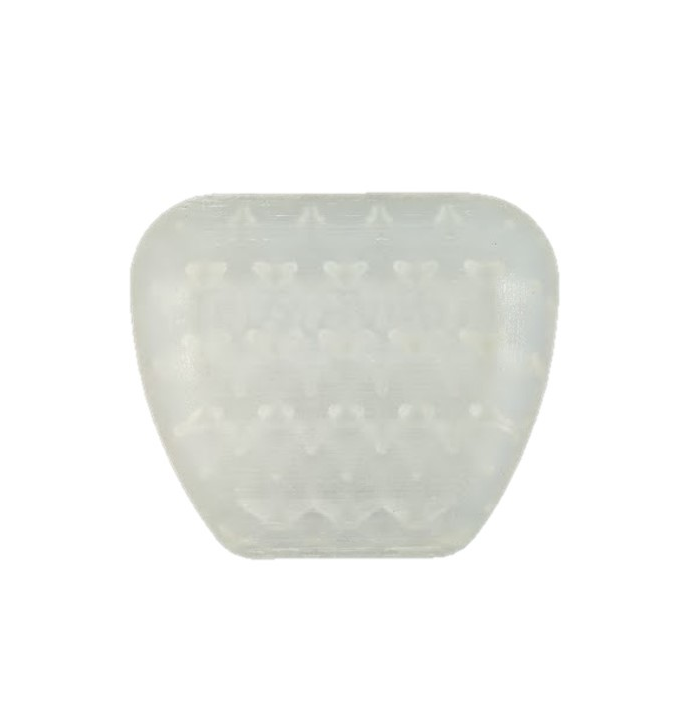
\includegraphics[scale=0.4]{../fig/eps/soft_finger.eps}}
\caption{球面化柔軟指}
\label{fig::soft_finger}
\end{figure}

\subsubsection{半球型柔軟指}
半球形柔軟指を\refig{semi_finger}に示す.
荷重が適切に測定できるようにラティス構造とセンサ部が接触する面の球面化を提案する.従来ではラティス構造とセンサ部は平面で接触しているため力の分散が考えられる測定困難であるとされたが接触面を球面化することにより荷重が集中し測定が可能になると考えられる.そこで球面化柔軟指(変更予定)	と名付けた指を\refig{semi_finger}に示す.半球形の把持部の中に先に述べた指と同じパラメータのラティス構造設計した.

\begin{figure}[h]
\centering
\subfloat[横]{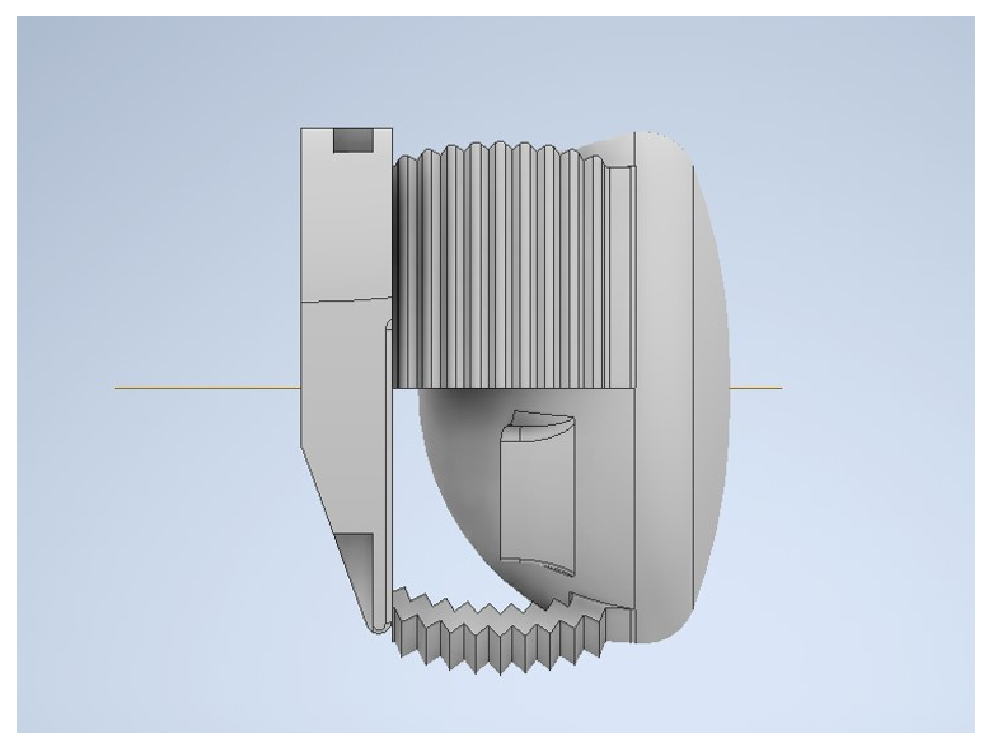
\includegraphics[scale=0.4]{../fig/eps/semi_finger.eps}}
\hspace{5mm}
\subfloat[正面]{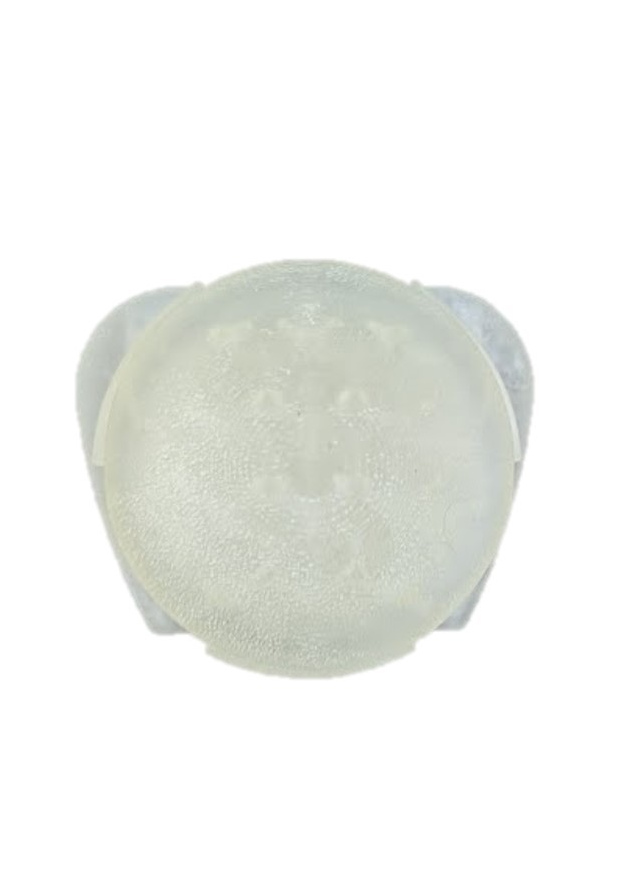
\includegraphics[scale=0.4]{../fig/eps/semi_finger_b.eps}}
\caption{球面化柔軟指}
\label{fig::semi_finger}
\end{figure}

\subsection{ラティス構造}
ラティス構造とは\refig{latice}に示す最小の繰り返し単位が周期的に繰り返される3次元構造で、機械的な強度を損なうことなく軽量化を可能とする\cite{latice}.ラティス構造の特徴として3次元構造の形状や周期のパラメータを変更することができ変形量や内部応答を制御することが可能である.本研究ではAutodesk社製のNetfabbを用いてラティス構造の作成を行いその時のパラメータを以下に示す.

\begin{figure}[b]
 \begin{center}
  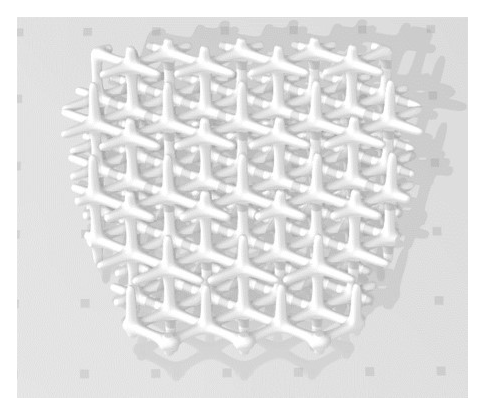
\includegraphics[scale=0.4]{../fig/eps/latice.eps}
 \caption{ラティス構造}
  \label{fig::latice}
 \end{center}
\end{figure}


\subsection{力覚センサ}
イナバゴム社のイナストマーを用いた.\refig{ina}に示す.イナストマーは感圧導電性エラストマー(加圧導電性ゴム)\cite{kanatsu}というゴムを利用した力覚センサである.絶縁性の高いゴム材料(1015~1018Ω)に導電性粒子(カーボン、金属粉、金属蒸着粉等)を一定の配合割合でほぼ均一に混ぜることで感圧導電性を付加している.

\begin{figure}[b]
 \begin{center}
  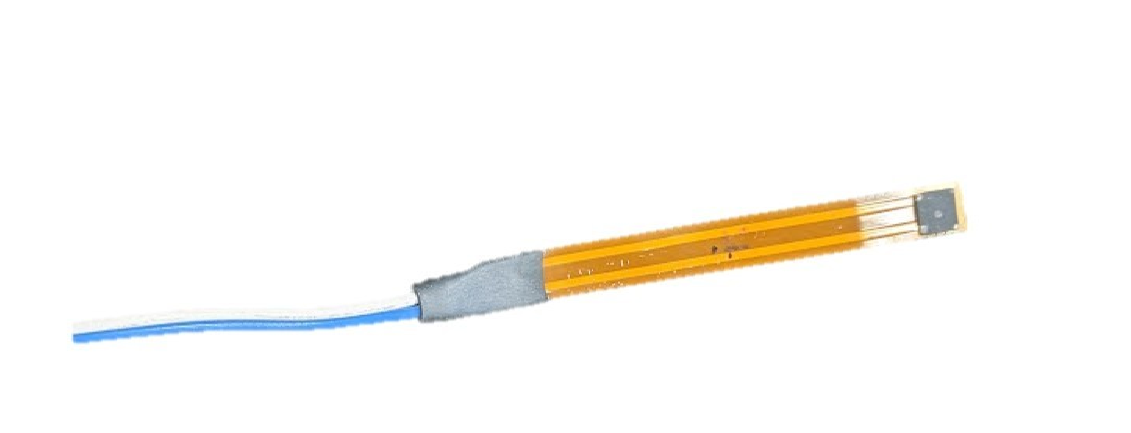
\includegraphics[scale=0.4]{../fig/eps/ina.eps}
 \caption{イナストマー}
  \label{fig::ina}
 \end{center}
\end{figure}

\subsubsection{動作原理}
感圧伝導性エラストマーが加圧されると内部の導電性粒子が次第に接触しはじめ導電経路が形成され電気抵抗値が低下する.また、減圧して無加圧にするとゴムの弾性による復元力で再度非接触状態に戻る.

	

\newpage